%%%%%%%%%%%%%%%%%%%%%%%%%%%%%%%%%%%%%%%%%%%%%%%%%%%%%%%%%%%%%%%%%%%%%%%%%%%%%
%%%
%%% File: thesis.tex, version 1.7, March 2021
%%%
%%% =============================================
%%% This file contains a template that can be used with the package
%%% cs.sty and LaTeX2e to produce a thesis that meets the requirements
%%% of the Computer Science Department from the Technical University of Cluj-Napoca
%%%%%%%%%%%%%%%%%%%%%%%%%%%%%%%%%%%%%%%%%%%%%%%%%%%%%%%%%%%%%%%%%%%%%%%%%%%%%

\documentclass[12pt,a4paper,twoside]{report}         
\usepackage{cs}
\usepackage[T1]{fontenc} 
\usepackage[utf8]{inputenc}
%\usepackage[romanian]{babel}              
\usepackage{times}
\usepackage{graphicx}
\usepackage{latexsym}
\usepackage{amsmath,amsbsy}
\usepackage{amssymb}
\usepackage[matrix,arrow]{xy}
\usepackage{ae,aecompl}
\usepackage{amstext}
\usepackage{graphics}
\usepackage{ae,aecompl}
\usepackage{algorithm}
\usepackage{color}
\usepackage{titlesec}
\usepackage{fancyhdr}
\usepackage{hyperref} 
%% decomentati linia urmatoare pentru e nu mai evidenția hiper legăturile pentru imprimare pe hârtie
%\hypersetup{hidelinks}
\usepackage{geometry}
\usepackage{lipsum}
\usepackage{enumitem}

\setlist{noitemsep,nolistsep}

\diplomathesis
\centerchapter
\singlespace
\newenvironment{definition}[1][Definition.]{\begin{trivlist}
\item[\hskip \labelsep {\bfseries #1}]}{\end{trivlist}}

%%%%%%%%%%%%%%%%%%%%%%%%%%%%%% Change the last element accordingly
\renewcommand{\thesisauthor}{Firstname LASTNAME}    %% Your first name(s) and family name.
\renewcommand{\thesismonth}{July}     %% The month of the licence session
\renewcommand{\thesisyear}{2022}      %% The year of the 
\renewcommand{\thesistitle}{LICENSE THESIS TITLE} % Title of the thesis
\renewcommand{\thesissupervisor}{scientific title Firstname LASTNAME} %% Supervisor
%%%%%%%%%%%%%%%%%%%%%%%%%%%%%%%%%%%%%
\newcommand{\makeThesisTitle}{\textbf{\thesistitletypesize \thesistitle}}
\newcommand{\makeThesisType}{\thesistypetypesize \thesistype}
\newcommand{\department}{\sffamily\bfseries\small FACULTY OF AUTOMATION AND COMPUTER SCIENCE} 
\renewcommand{\thesistype}{LICENSE THESIS}
\newcommand{\uline}[1]{\rule[0pt]{#1}{0.4pt}}
%\renewcommand{\thesisdedication}{Părinților mei}

% Headings pentru folie de capăt

 \geometry{
	a4paper,
	total={159.2mm,246.2mm},
	left=25.4mm,
	top=25.4mm,
}


\begin{document}
%\frontmatter
%%%%%%%%%%% Stil pentru paginile de capăt
\pagestyle{fancy}
\setlength{\voffset}{-10pt}
\setlength\headheight{70.0pt}
%\addtolength{\textheight}{-80.0pt}
\renewcommand{\headrulewidth}{0pt}
\chead{%
	
\includegraphics[width=\textwidth]{figs/AntetUTCNEng.pdf}
}
\cfoot{}
\lfoot{}
\rfoot{}
%\pagestyle{headings}
%%%%% Thesis title page %%%%%%%%%%%%%%%%%%%%%%%%
\begin{center}
	{\department}
	
	\vspace{4cm}
	\makeThesisTitle %LICENSE THESIS TITLE
	~\\~\\
	
	\makeThesisType
	
	~\\\vspace{6.5cm}
	
	\begin{tabular}{p{.3\linewidth}p{.5\linewidth}}
		{\hfill Graduate:} & {\bf \thesisauthor} \\
		&\\
		{\parbox[t]{\linewidth}{\hfill Supervisor:}}& {\bf \thesissupervisor}\\
	\end{tabular}
	
	\vspace{3cm}
	{\bf \thesisyear}
\end{center}
%%%%%%%%%%%%%%%%% end of thesis title page %%%%%%%%%%%%%%%%%%%%%%%%%%%%%%%%%%%%
\newpage
%%%%%%% Proposal page %%%%%%%%%%%%%%%%%%%%%%%%%%%%%%%
\begin{center}
	{\department}
\end{center}
\vspace{0.5cm}

%\begin{small}
\begin{tabular}{p{7cm}p{8cm}}
	%\hspace{-1cm}& VIZAT,\\
	\hspace{-1cm}DEAN, & HEAD OF DEPARTAMENT,\\
	\hspace{-1cm}{\bf Prof. dr. ing. Liviu MICLEA} & {\bf Prof. dr. ing. Rodica POTOLEA}\\  
\end{tabular}

\vspace{2cm}

\begin{center}
	Graduate: {\bf \thesisauthor}
	
	\vspace{1cm}
	
	{\bf \thesistitle}
\end{center}

\vspace{5mm}

\begin{enumerate}
	\item {\bf Project proposal:} {\it Short description of the license thesis  and initial data}
	\item {\bf Project contents:} {\it (enumerarea părților componente) Example: : (enumerate the main component parts) Presentation page, advisor's evaluation, title of chapter 1, title of chapter 2, …, title of chapter n, bibliography, appendices .}
	\item {\bf Place of documentation:} {\it Example}: Technical University of Cluj-Napoca, Computer Science Department 
	\item {\bf Consultants:}
	\item {\bf Data of issue of the proposal:} November 1, 2021 %%%%%%%%%%%%% Modificați corespunzător
	\item {\bf Data od delivery :} July 8, 2022 %%%%%%%%%%%%%%% Modificați corespunzător
\end{enumerate}
\vspace{1.2cm}

\hspace{6cm} Graduate: \uline{6cm} 

\vspace{0.5cm}
\hspace{6cm} Supervisor: \uline{5cm} 
\newpage
%%%%%%%%%%%%%%%%%% End of proposal page
%%%%%%%%% Page with declaration %%%%%%%%%%%%%%%%%%%%%%%%%%%%%%%%%%%%%%%%%%
\begin{center}
	{\department}
\end{center}
\vspace{1cm}
\begin{center}
	{\bf Declarație pe proprie răspundere privind\\ 
		autenticitatea lucrării de licență}
\end{center}
\vspace{1cm}

\begin{minipage}{\linewidth}
	\indent Subsemnatul(a) \uline{.73\linewidth},
	\uline{.82\linewidth}
	legitimat(ă) cu\\ \uline{4cm} seria \uline{3cm} nr. \uline{6.3cm}
	CNP \uline{9cm}, autorul lucrării\
	\uline{\linewidth}
	\uline{\linewidth}
	elaborată în vederea susținerii examenului de finalizare a studiilor de licență la Facultatea de Automatică și Calculatoare, Specializarea \uline{7cm} din cadrul Universității Tehnice din Cluj-Napoca, sesiunea \uline{4cm} a anului universitar \uline{3cm}, declar pe proprie răspundere, că această lucrare este rezultatul propriei activități intelectuale, pe baza cercetărilor mele și pe baza informațiilor obținute din surse care au fost citate, în textul lucrării și în bibliografie.\\
	\hspace*{8mm} Declar, că această lucrare nu conține porțiuni plagiate, iar sursele bibliografice au fost folosite cu respectarea legislației române și a convențiilor internaționale privind drepturile de autor.\\
	\hspace*{8mm} Declar, de asemenea, că această lucrare nu a mai fost prezentată în fața unei alte comisii de examen de licență.\\
	\hspace*{8mm} În cazul constatării ulterioare a unor declarații false, voi suporta sancțiunile administrative, respectiv, \emph{anularea examenului de licență}.
\end{minipage}
\vspace{1.5cm}

Data \hspace{8cm} Nume, Prenume

\vspace{0.5cm}

\uline{3cm} \hspace{5cm} \uline{5cm}

\vspace{1cm}
\hspace{9.4cm}Semnătura
\newpage
%%%%%%%%%%%%%%%%%%% end of page with declaration % the first 3 pages
%%%%%%%%%%%%%%%%% Advices page to remove
\thispagestyle{empty}
\thispagestyle{empty}
\begin{center}\large
	General Advice
\end{center}
~\\

{\color{red}\large{\bf READ FIRST} (this page should be removed from the final version)}:\\
\begin{enumerate}
	\item	If you print the thesis on paper, the three preceding pages (title page, summary page and declaration) should be printed on separate pages (one-side) and should be included in the printed paper. The summary page (the second one) must be signed by the graduate and the supervisor. The date on the declaration should be the date when the thesis is handed to the commissions’ secretary.
	\item	On the title page, you should include the correct scientific title of your supervisor (use the Department web pages to find that).
	\item Every chapter begins on a new page.
	\item Do not change page margins.
	\item Obey the other instructions provided in every chapter.
	\item This template obeys all the formatting rules.
	\item We included the \verb+hyperref+ package to generate navigation links. To produce  a version for printing on paper uncomment the line containing \verb+%\hypersetup{hidelinks}+
	located in the beginning of the main file \verb+thesis_rom.tex+. 
\end{enumerate}
 
\newpage
%%%%%%%%%%%%%%%%%% edn of advices page
\pagestyle{fancy}
\setlength\headheight{16.0pt}
\renewcommand{\chaptermark}[1]{\markboth{\chaptername~\thechapter.~#1}{}}
\renewcommand{\sectionmark}[1]{\markright{\thesection\ #1}}
\renewcommand{\headrulewidth}{0.4pt}
\lhead{}
\chead{%
	\leftmark\rightmark
}
\chead{}
\cfoot{\thepage}
\lfoot{}
\rfoot{}

%%%%%%%%%%%% Table of contents
\pagenumbering{roman}
\setcounter{page}{1}

\newpage

\tableofcontents

\newpage

%\listoftables
%\listoffigures

\pagenumbering{arabic}
\setcounter{page}{1}


\titleformat{\chapter}[hang] 
{\normalfont\Large\bfseries}{\chaptertitlename\ \thechapter.}{1em}{}
\titleformat{\section}[hang] 
{\normalfont\large\bfseries}{\thesection.}{1em}{}
\titleformat{\subsection}[hang] 
{\normalfont}{\thesubsection.}{1em}{}

\chapter{Introduction - Project Context}\label{ch:context}
\pagestyle{fancy}

{\color{blue}\noindent About 5\% of the paper..\\}
\noindent This chapter will present:

\begin{itemize}
	\item Project context
	\item Specification of the precise domain of the license thesis
\end{itemize}




\section{Project context}\label{sec:context}

\subsection{Subsection title}

Each table used in this document is labeled as Table x.y, where x represents the chapter number, and y shows the table number within the current chapter. Leave a blank line between and after each table, relative to the adjacent paragraphs.
To refer to a table useL ~\ref{tab:nonlin}.

\begin{table}[ht]
	\caption{Results}
	\centering                          % centered table
	\begin{tabular}{|c|c|c|c|}          % 4 centered columns 
		\hline
		Case & Method\#1 & Method\#2 & Method\#3 \\ [0.5ex]   % inserare tabel
		%heading
		\hline                              % horizontal simple line
		1 & 50 & 837 & 970 \\               % table body
		2 & 47 & 877 & 230 \\
		3 & 31 & 25 & 415 \\[1ex]           % [1ex] adds vertical space
		\hline                              
	\end{tabular}
	% titlul tabelului
	\label{tab:nonlin}                % \label{table:nonlin} introduce eticheta folosita pentru referirea tabelului in text; referirea in text se va face cu \ref{table:nonlin}
\end{table}

Each figure used in the document must be referred within the text (ex: in Figure x.y the system components are presented... ) and labeled. The labeling must be as Figure x.y where x represents the chapter number, and y shows the number of the figure within the current chapter. 
Use the following method to refer an image ~\ref{fig:imag}.

\begin{figure}[ht]
	\centering
	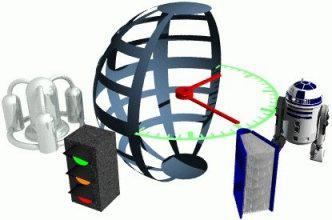
\includegraphics[]{figs/test.jpg}
	\caption{}
	\label{fig:imag}
\end{figure}

Each new chapter starts on a new page.

\vspace{10pt}

\lipsum[1-15]
\newpage % \chapter{Introdution}

\chapter{Project Objectives}\label{ch:obiective}
\pagestyle{fancy}

{\noindent\color{blue}This chapter should take about 10\% of the paper.\\}

The project theme must be described in this chapter (as a research/design proposal, clearly formulated, with clear objectives – 2-3 pages – and, possibly, some explanatory figures).



\section{Section 1}
\section{Section 2}

\lipsum[2-11] % \chapter{Obiectivele Proiectului}

\chapter{Bibliographic Research}\label{ch:studiubib}

\pagestyle{fancy}


{\color{blue}\noindent This chapter should take about 15\% of the paper.\\}

Bibliographic research has as an objective the establishment of the references for the project, within the project domain/thematic. While writing this chapter (in general the whole document), the author will consider the knowledge accumulated from several dedicated disciplines in the second semester, 4th year (Project Elaboration Methodology, etc.), and other disciplines that are relevant to the project theme.

Each reference \textbf{must} be cited within the document. Please look at the examples below (depending on the project theme, the presentation of a method/application can vary).

Referințele are included in the Bibliography chapter. 

References can by managed with \href{https://www.jabref.org/}{JabRef}, an application which can be downloaded from \url{https://www.jabref.org/#download}

Examples of what should be included in each type of reference can be found \href{https://libguides.nps.edu/citation/ieee-bibtex}{here}.

About common errors found in online libraries of references you can read at \href{https://www.ece.ucdavis.edu/~jowens/biberrors.html}{here}

In paper \cite{BellucciLZ04} the authors present a detection system for moving obstacles based on stereovision and ego motion estimation (note that this is not true about that the article contents). The method is … discus the algorithms, data structures, functionality, specific aspects related to the project theme, etc…. Discussion: pros and cons. Some bib templates can be used: ~\cite{BellucciLZ04} for conferences, ~\cite{AntoniouSBDB07} for journal articles and ~\cite{russell1995artificial} for citing books.  References to applications or online resources (web pages) must include at least a short relevant description in addition to the link ~\cite{webpage}, and other information is available (authors, year, etc.). References that contain only the link to the online resource will be placed in the page footer

In chapter ~\ref{ch:analysis} from ~\cite{strunk} the similar-to-my-project-theme algorithm is presented, with the following features…



\section{Some section}

\subsection{Some sub-section}
\lipsum[2-9]
 % \chapter{Studiu Bibliografic}

\chapter{Analysis and Theoretical Foundation}
\label{ch:analysis}
\pagestyle{fancy}

{\color{blue} Together with the next chapter takes about 60\% of the whole paper.\\}

The purpose of this chapter is to explain the operating principles of the implemented application.
Here you write about your solution from a theory standpoint – i.e. you explain it and demonstrate its theoretical properties/value, e.g.:
\begin{itemize}
	\item used or proposed algorithms,
	\item used protocols,
	\item abstract models,
	\item logic explanations/arguments concerning the chosen solution,
	\item logic and functional structure of the application, etc.
\end{itemize}


~\\\parbox[c]{\textwidth}{\color{red}\bfseries

YOU SHOULD NOT write about implementation. 
	
YOU SHOULD NOT copy/paste information on technologies and other alike from various sources, which do not pertain to your project (no fillers, please!).
}


\section{Section 1}
\section{Section 2}
 % \chapter{Analiză și Fundamentare Teoretică}

\chapter{Detailed Design and Implementation}
\pagestyle{fancy}

{\color{blue}Together with the previous chapter takes about 60\% of the paper.\\}

The purpose of this chapter is to document the developed application such a way that it can be maintained and developed later. A reader should be able (from what you have written here) to identify the main functions of the application.
The chapter should contain (but not limited to):
\begin{itemize}
	\item a general application sketch/scheme,
	\item a description of every component implemented, at module level,
	\item class diagrams, important classes and methods from key classes.
\end{itemize}

\section{Section 1}
\section{Other section}
\lipsum[10-20] % \chapter{Proiectare de Detaliu și Implementare}

\chapter{Testing and Validation}
\pagestyle{fancy}

{\noindent\color{blue}This chapter should take about 5\% of the paper.}

\section{Section 1}
\section{Section 2}

\lipsum[1-5] % \chapter{Testare și Validare}

\chapter{User’s manual}
\pagestyle{fancy}

In the section describing the installation procedure you should detail the hardware and software resources needed for installing and running the application, and a step by step description of how your application can be deployed/installed. An administrator should be able to perform the installation/deployment based on your instructions.
In the section for the user you should describe how to use the application from the point of view of a user with no inside technical information; this should be adorned with screen shots and a step-wise explanation of the interaction. Based on user's manual, a person should be able to install and use your product.


\section{Section 1}
\section{Section 2}

\lipsum[1-10] % \chapter{Manual de Instalare și Utilizare}

\chapter{Conclusions}
\pagestyle{fancy}

{\noindent\color{blue}This chapter should take about 5\% of the paper.}

In this chapter you should include:
\begin{itemize}
	\item A summary of your contributions/achievements,
	\item A critical analysis of the results achieved,
	\item A description of the possibilities of improvements/further development.
\end{itemize}

\section{Section 1}
\section{Section 2}

 % \chapter{Concluzii}


\bibliographystyle{IEEEtran} 
\bibliography{thesis}%same file name as for .bib

\appendix
\chapter{Relevant code sections}
\pagestyle{fancy}

\begin{verbatim}
 /** Maps are easy to use in Scala. */
object Maps {
  val colors = Map("red" -> 0xFF0000,
                   "turquoise" -> 0x00FFFF,
                   "black" -> 0x000000,
                   "orange" -> 0xFF8040,
                   "brown" -> 0x804000)
  def main(args: Array[String]) {
    for (name <- args) println(
      colors.get(name) match {
        case Some(code) =>
          name + " has code: " + code
        case None =>
          "Unknown color: " + name
      }
    )
  }
}
\end{verbatim}

\chapter{Other relevant info (proofs etc.)}


\chapter{Published papers (if any)}


\end{document}
